\section{\Tool design}
\label{sec:design}
\Tool consists of a series of analysis that
judges whether a given loop belongs to any root cause type discussed in
Section \ref{sec:study_tax}.
Its design
follows the following principles.
\begin{itemize}
\item Failure diagnosis, not bug detection. \Tool will be  
used together with other performance diagnosis tools \cite{SongOOPSLA2014}
and focus on a small
number of loops that are most correlated with a specific performance symptom,
instead of being applied to the whole program. Therefore, we will have different
design trade-offs in terms of coverage and accuracy, comparing with 
bug detection tools.

\item Static-dynamic hybrid analysis. Static analysis alone
will not be able to provide all the needed information to judge whether
a loop is inefficient. However, 
dynamic analysis alone will incur too much overhead.
Therefore, we use a hybrid approach throughout our design.

\item Sampling. Loop-related 
performance problems have the unique nature of repetitiveness, which make 
them a natural fit for random sampling. We will design different
sampling schemes for different analysis.
\end{itemize}

\subsection{Resultless Checker}
\label{sec:workless}

Our resultless checker includes two parts. First, we use static analysis
to figure out which are the side-effect instructions in a loop and hence
decide whether a loop belongs to 0*, 0*1?, [0$|$1]*, or 1*. Second, to
accurately determine 0*1? and [0$|$1]* loops, we use
dynamic analysis to figure out what portion of loop iterations are
resultless at run time.
%, which will help decide whether the loop is indeed
%inefficient.

%\begin{figure}[ht]
%\center
%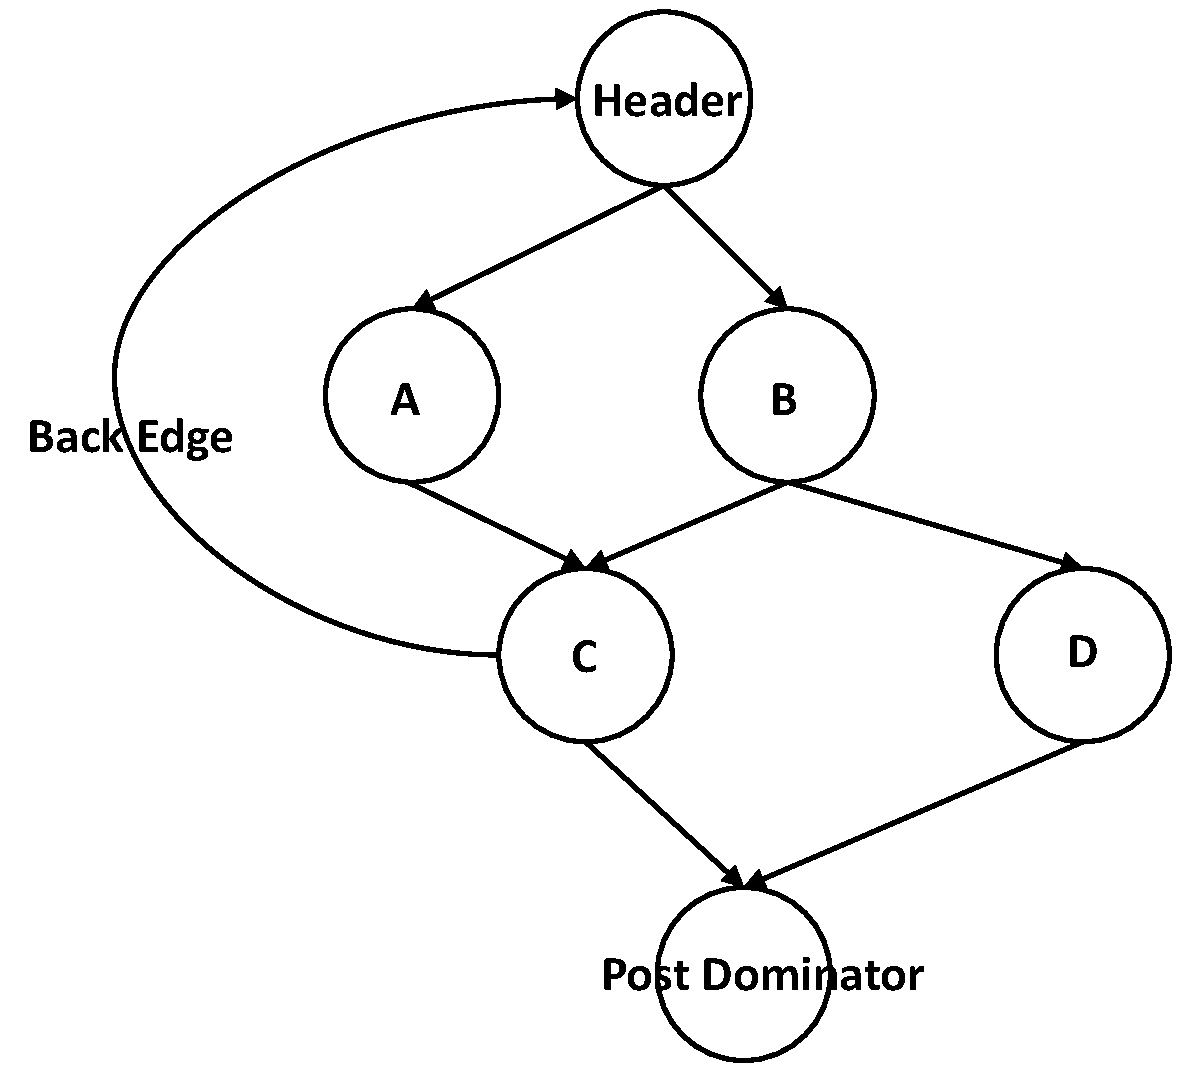
\includegraphics[width=0.7\linewidth]{figures/workless.pdf}
%\caption{Examples for different types of basic blocks inside a loop}
%\label{fig:block_type}
%\end{figure}

\subsubsection{Static Analysis}
\label{sec:s_workless}

\Tool first identifies side-effect instructions that write to
variables defined outside the loop. 
\Tool analyzes all functions called
by a loop directly or indirectly --- a function $F$ that updates variables
defined outside $F$ makes the corresponding call statement in $F$'s
caller a side-effect instruction.
We consider all calls to library functions or through function pointers 
as having side effects, 
unless the library functions are specially marked by us in a white list.

\Tool then categorizes loops into four types.
Given a natural loop $l$, when $l$
contains at least one side-effect instruction along every path that
starts from the loop header and ends at the loop header, it is a 1* loop;
if there exists at least one side-effect instruction inside $l$, but not on
every path,
it is a [0$|$1]* loop; if there is no side-effect instructions inside $l$,
$l$ is either a 0* or a 0*1? loop.
In the last case, \Tool further checks all the loop exit-blocks. If there 
exists an exit-block of $l$ that contains a side-effect instruction and is  
post-dominated by another exit-block of $l$, this is a 0*1? loop.
For example, line 5 in Figure \ref{fig:Mozilla347306} is such an exit block.
Otherwise, $l$ is a 0* loop.

Note that since the 1* pattern contains the least amount of information
about computation \textit{inefficiency}, \Tool will not report a loop's
root-cause type as 1*, if more informative root-cause type is identified 
for this loop (e.g., cross-iteration or cross-loop redundancy).

%TODO Shan will rewrite the next two paragraphs
\subsubsection{Dynamic Monitoring}
\label{sec:d_workless}

Except for 0*, none of the other three type of loops are inefficient for sure.
We need dynamic analysis to figure out what portion of loop iterations are
resultless at run time, which will help decide whether the loop worths fixing.

For a 0*1? loop, since it only generates results in the last iteration, we 
only need to know the total number of loop iterations 
to figure out the 
\textit{resultless rate} of the loop. The implementation is straightforward
--- we initialize a local counter to be 0 in the pre-header of the loop; we 
increase the counter by 1 in the loop header to count the number of 
iterations; we dump that counter to log when the loop exits.

For [0$|$1]*, we need to count not only the total number of iterations, but
also the exact number of iterations that execute side-effect instructions
at run time. 
To do that, our instrumentation uses a local boolean variable 
\texttt{HasResult} to represent whether one iteration have side effect or not. 
\texttt{HasResult} is set to \texttt{False} in the loop header, and set to
\texttt{True} after each side-effect instruction. It will be used to help
count the number of side-effect iterations. For performance concerns,
before instrumenting side-effect blocks, we check whether there are 
post-domination relation between each pair of side-effect blocks. 
If both block A and block B are side-effect blocks and block A post-dominates 
block B, we only instrument block A to update \texttt{HasResult}. 

\comment{
We could speed up the above counting using sampling. However, since the 
run-time overhead of the above counting is low, as shown in Section 
\ref{sec:experiment}, our current prototype of \Tool does 
not use sampling for this part of run-time analysis.
}

%\subsubsection{Sampling}
%We calculate the average iteration number 
%and the ratio of working iteration based on a separated 
%process from on-line branch sampling discussed in~\cite{SongOOPSLA2014}.
%We need to instrument the buggy program and re-execute it by using bug-triggering input. 
%In the future, we could design an algorithm to calculate the two resultless metrics 
%based on branch sampling reports to get rid of the extra instrumentation and the extra bad run.   

\comment{
\subsubsection{Limitations}
\label{sec:l_workless}
When callee may have side effect, we will consider it will have side effect in the caller side, 
and do not consider the real execution inside callee. This could bring false negatives, 
because we could miss resultless cases, 
where side effect instructions inside callee do not execute. 
Experiments results in Section~\ref{sec:experiment} show that this is not a big issue, 
since we do not miss any resultless bugs.  

Second, our dynamic instrumentation does not consider concurrent execution of the monitored loop, 
because most of buggy loops we study only execute in one single thread. 
When the monitored loop is executed in multi-thread, like loop marked with omp pragma, we need to synchronize updates to global variables. 
}
